\chapter{Metodología}
\label{cap:metodologia}

En este capítulo se describe el proceso de obtención de la velocidad de vehículos a partir de secuencias de imágenes. Para realizar esta tarea se recopiló un conjunto de datos (\textit{dataset}) suficiente para  realizar la tarea de estimación de la velocidad,  a partir del \textit{dataset}. El problema de obtención de la velocidad fue dividido en tres procesos principales (extracción de características, modelo predictivo y obtención de la velocidad). Para la generación del \textit{dataset} fue necesario ir físicamente a una vía terrestre. Una vez en la vialidad, se utilizó una cámara para capturar la secuencias de imágenes y un radar para medir la velocidad del vehículo. El proceso de extracción de características parte de los videos (secuencias de imágenes) para después aplicar técnicas de aprendizaje profundo. Resultando en un archivo con extensión csv con las características esenciales con los vehículos en cuestión. A partir del archivo con extensión csv se aplicaron técnicas estadísticas de correlación con la finalidad de relacionar la distancia en píxeles con una distancia en metros. Para posteriormente estimar la velocidad del vehículo (obtención de la velocidad). 


La metodología completa se divide en dos grandes procesos como lo muestra la Figura \ref{fig:MetodologiaDF}. El proceso de obtención del conjunto de datos, que consistió en la generación de muestras de campo con las cuales se realizó esta investigación. Y a partir de las muestras recolectadas se realizó el proceso de obtención de la velocidad.

\begin{figure}[H]
    \centering
    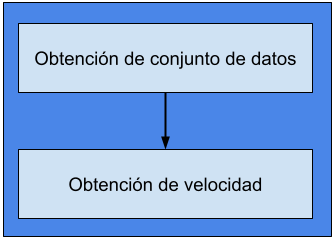
\includegraphics[width=0.5\textwidth]{Metodologia/imgs/ProcesoObtencionVelocidad.png}
    \caption{Proceso de obtención de la velocidad.}
    \label{fig:MetodologiaDF}
\end{figure}


\section{Obtención de conjunto de datos}


La obtención del conjunto de datos se divide en dos etapas, la primera etapa corresponde a la toma de muestras, la cual implica ir al lugar con flujo constante de vehículos para obtener la mayor cantidad de datos. La segunda etapa es la limpieza de las muestras con la cual se busca solo tomar en cuenta los vehículos a los que se logró tomar correctamente la velocidad.
La Figura \ref{fig:DFCreacionCD} muestra las dos etapas internas con las que cuenta la obtención de conjunto de datos.

\begin{figure}[H]
    \centering
    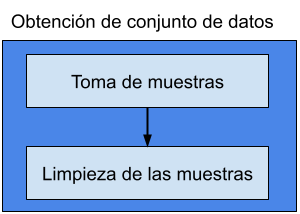
\includegraphics[width=0.5\textwidth]{Metodologia/imgs/ObtencionConjuntoDatos.png}
    \caption{Proceso de obtención de conjunto de datos.}
    \label{fig:DFCreacionCD}
\end{figure}


%%%%%%%%%%%%%%%%%%%%%%%%%%%%%%%%%%%%%%%%%%%%%%%%%%%%%%%%%%%%%%%%%%%%%%%%%%%%%%%%
%%%%%%%%%%%%%%%%%%%%%%%%%%%%%%%%%%%%%%%%%%%%%%%%%%%%%%%%%%%%%%%%%%%%%%%%%%%%%%%%
%%%%%%%%%%%%%%%%%%%%%%%%%%%%%%%%%%%%%%%%%%%%%%%%%%%%%%%%%%%%%%%%%%%%%%%%%%%%%%%%
%%%%%%%%%%%%%%%%%%%%%%%%%%%%%%%%%%%%%%%%%%%%%%%%%%%%%%%%%%%%%%%%%%%%%%%%%%%%%%%%
%%%%%%%%%%%%%%%%%%%%%%%%%%%%%%%%%%%%%%%%%%%%%%%%%%%%%%%%%%%%%%%%%%%%%%%%%%%%%%%%

\subsection{Toma de muestras}

Para la toma de muestras se requirió de dos dispositivos con los cuales se busca la extracción del conjunto de datos que posteriormente se utilizará como entrenamiento de los modelos predictivos. Uno de los dispositivos es el radar Bushnell (Figura \ref{fig:RadarVelocidad}) el cual tiene una precisión de +/- 1.6 kilómetros por hora.

\begin{figure}[H]
    \centering
    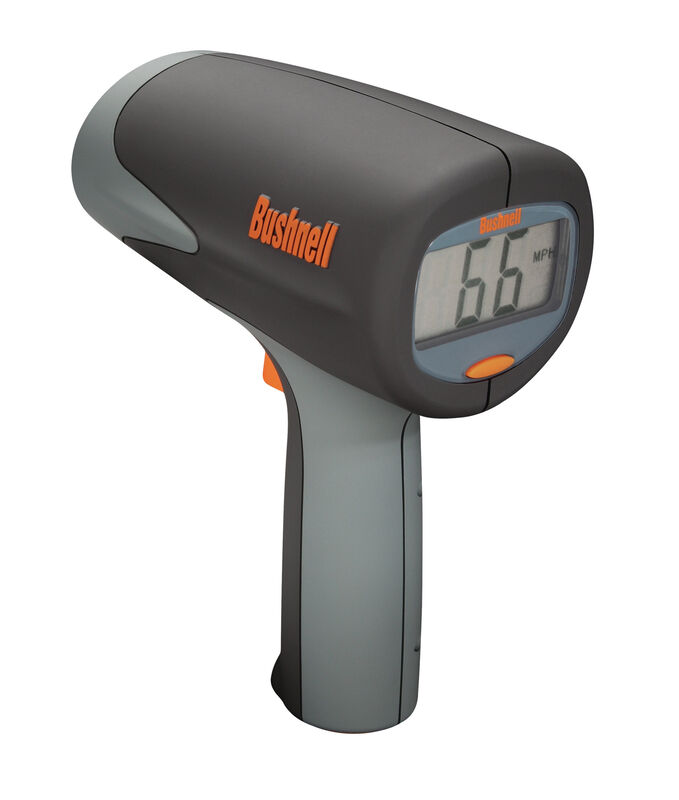
\includegraphics[width=0.4\textwidth]{Metodologia/imgs/bushnell.jpg}
    \caption{Radar de velocidad Bushnell(\cite{bushnell}).}
    \label{fig:RadarVelocidad}
\end{figure}

Mientras que el otro dispositivo es una cámara de video, la cual puede ser un dispositivo especializado para esta tarea o cualquier otro dispositivo capaz de grabar video. 
Las configuraciones mínimas pueden ser una resolución de 854 x 480 a 30 fotogramas por segundo. Sin embargo, hay que tomar en cuenta que al tener una resolución baja se puede perder calidad en la imagen y tomar un área menor a la deseada. Mientras que tener fotogramas tan bajos ocasionará perder vehículos que pasan a una velocidad más alta.
Por otro parte al aumentar la resolución y los fotogramas por segundo ocasiona que al sistema le tome más tiempo procesar el video. Para este caso se utilizó la cámara de Smartphones un Xiaomi Redmi Note 7 y un iPhone X configurados a 60 FPS y una resolución de Full HD (1920 x 1080 pixeles).

Existe un cuidado especial a la hora de posicionar la cámara, ya que no se quiere que los experimentos sean considerados como cálculos de velocidad en 2D, para esto la toma de muestras se realizó en un lugar donde el tráfico vehicular pase con cierto grado de inclinación, sin apuntar la cámara directamente al costado de donde pasan los vehículos, como muestra la Figura \ref{fig:LugarMuestrasDataset}.

\begin{figure}[H]
    \centering
    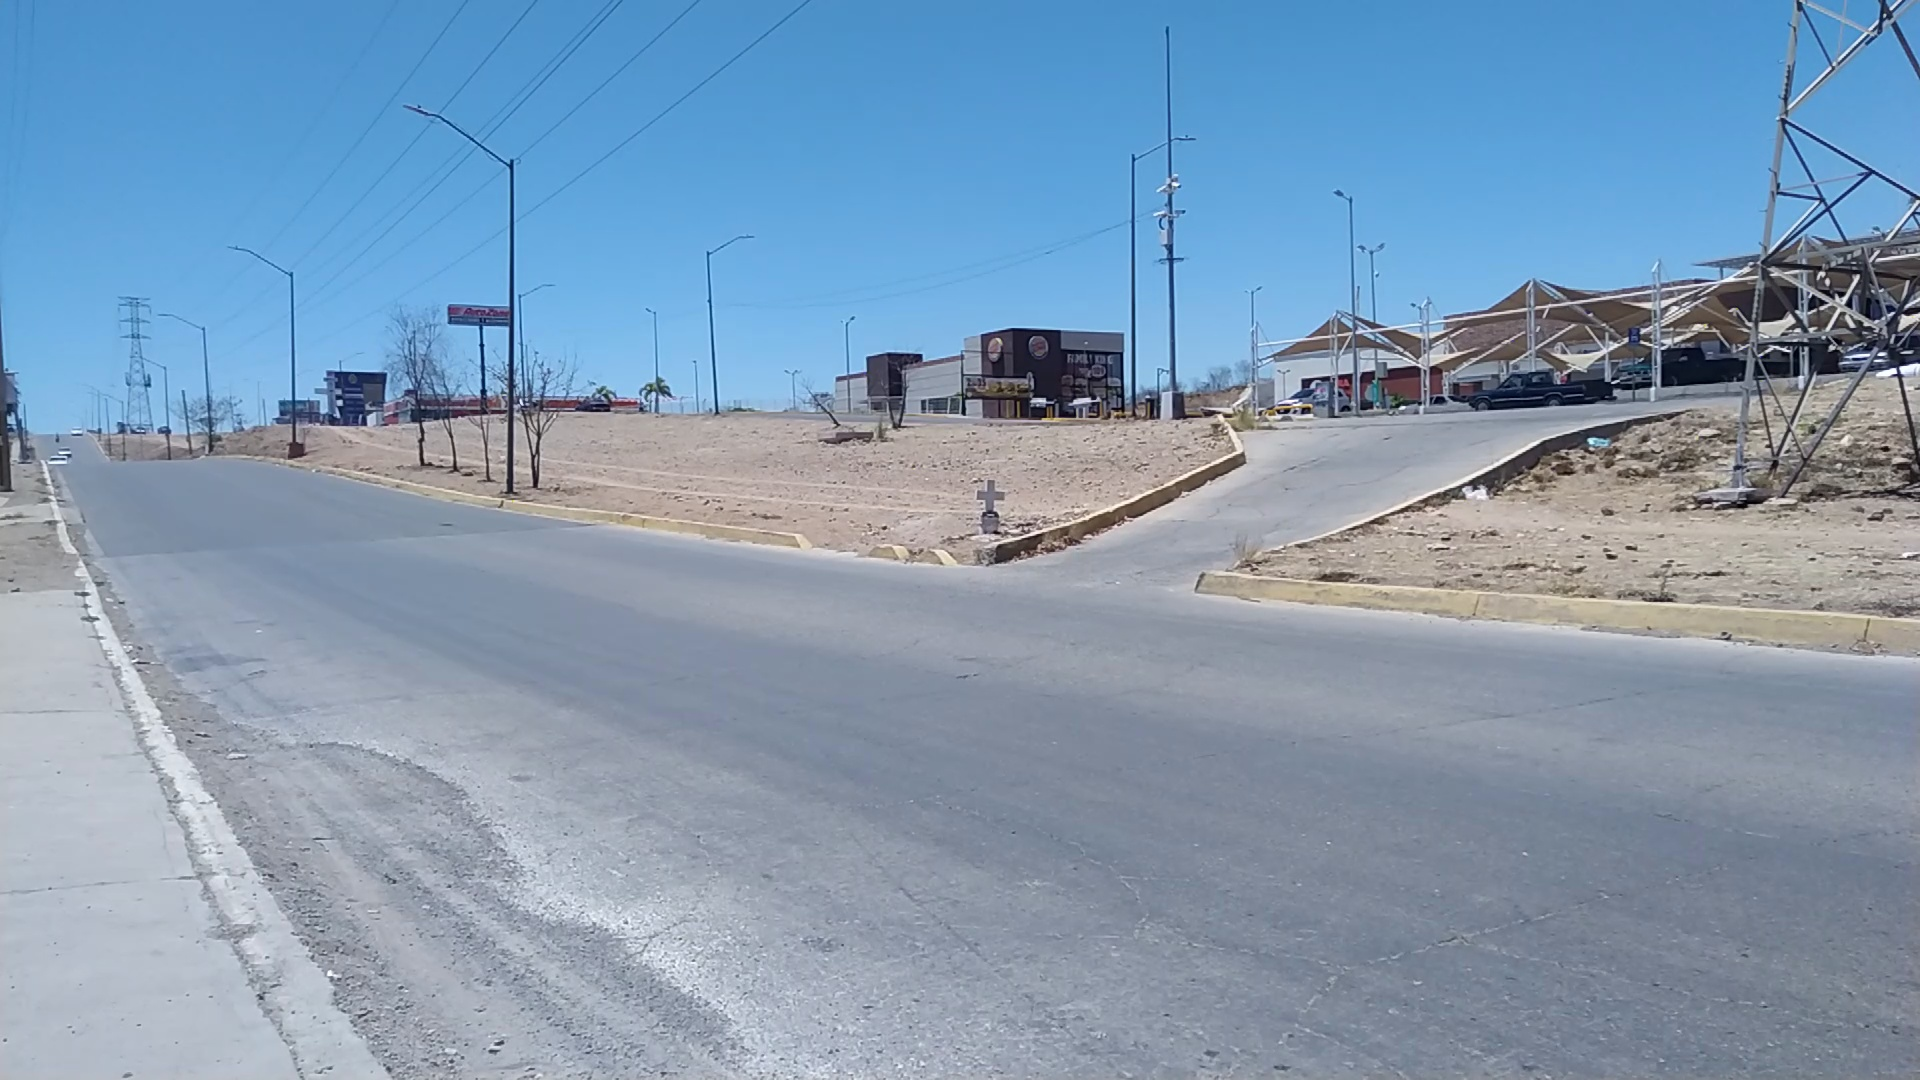
\includegraphics[width=0.8\textwidth]{Metodologia/imgs/LugarMuestras.jpg}
    \caption{Lugar donde se tomaron las muestras.}
    \label{fig:LugarMuestrasDataset}
\end{figure}

Cabe mencionar que por practicidad, el proceso de toma de muestras fue realizado, en un mismo lugar de la ciudad de Culiacán, Sinaloa.

Dado que la cámara y el radar de velocidad son dispositivos que no están sincronizados entre sí, fue necesario la implementación de un mecanismo para asociar la lectura del radar con la toma del video.

%%%%%%%%%%%%%%%%%%%%%%%%%%%%%%%%%%%%%%%%%%%%%%%%%%%%%%%%%%%%%%%%%%%%%%%%%%%%%%%%
%%%%%%%%%%%%%%%%%%%%%%%%%%%%%%%%%%%%%%%%%%%%%%%%%%%%%%%%%%%%%%%%%%%%%%%%%%%%%%%%
%%%%%%%%%%%%%%%%%%%%%%%%%%%%%%%%%%%%%%%%%%%%%%%%%%%%%%%%%%%%%%%%%%%%%%%%%%%%%%%%
%%%%%%%%%%%%%%%%%%%%%%%%%%%%%%%%%%%%%%%%%%%%%%%%%%%%%%%%%%%%%%%%%%%%%%%%%%%%%%%%
%%%%%%%%%%%%%%%%%%%%%%%%%%%%%%%%%%%%%%%%%%%%%%%%%%%%%%%%%%%%%%%%%%%%%%%%%%%%%%%%

\subsection{Limpieza de las muestras}

Una vez tomadas las muestras, fue necesario realizar una limpieza de los datos, estos son, los vehículos a los que se les detectó la velocidad utilizando el radar. Con la limpieza de los datos se busca eliminar los vehículos a los que no se les tomo la velocidad y dejando solo aquellos que si fueron considerados.

La toma de las muestras se realizá a partir de dos dispositivos que no están especializados para esta tarea (Cámara de video y radar de velocidad), la limpieza de las muestras ayuda a combinar la información de ambos dispositivos realizando una inspección visual de los videos, en la cual se identifica el segundo del video en el que pasa el vehículo de interes, la velocidad detectada por el radar, el carril por el cual viaja el vehículo y una descripción del vehículo para futuras referencias. Estos cuatro datos son guardados en un archivo de texto separado por comas (csv) el cual servirá de entrada para el siguiente paso en la metodología.

Determinar la velocidad es una tarea que necesita el tiempo y la distancia que toma un vehículo en pasar de un lugar a otro. Para esto el sistema necesita ser configurado con un punto de entrada y un punto de salida en el eje X. A partir de ahora a estos dos puntos se les llamará simplemente por punto A y punto B.  Los puntos A y B deben ser colocados de manera que los vehículos deben pasar completamente por cada uno de ellos. Además, cada una de las muestras deben tener diferentes valores para los puntos A y B, sin embargo, para este caso no fue necesario implementar diferentes valores, ya que todos los videos fueron tomados en el mismo lugar. La Figura \ref{fig:LugarLimites} muestra donde fueron colocados los puntos A y B en las muestras, denotados por dos lineas azules verticales.

\begin{figure}[H]
    \centering
    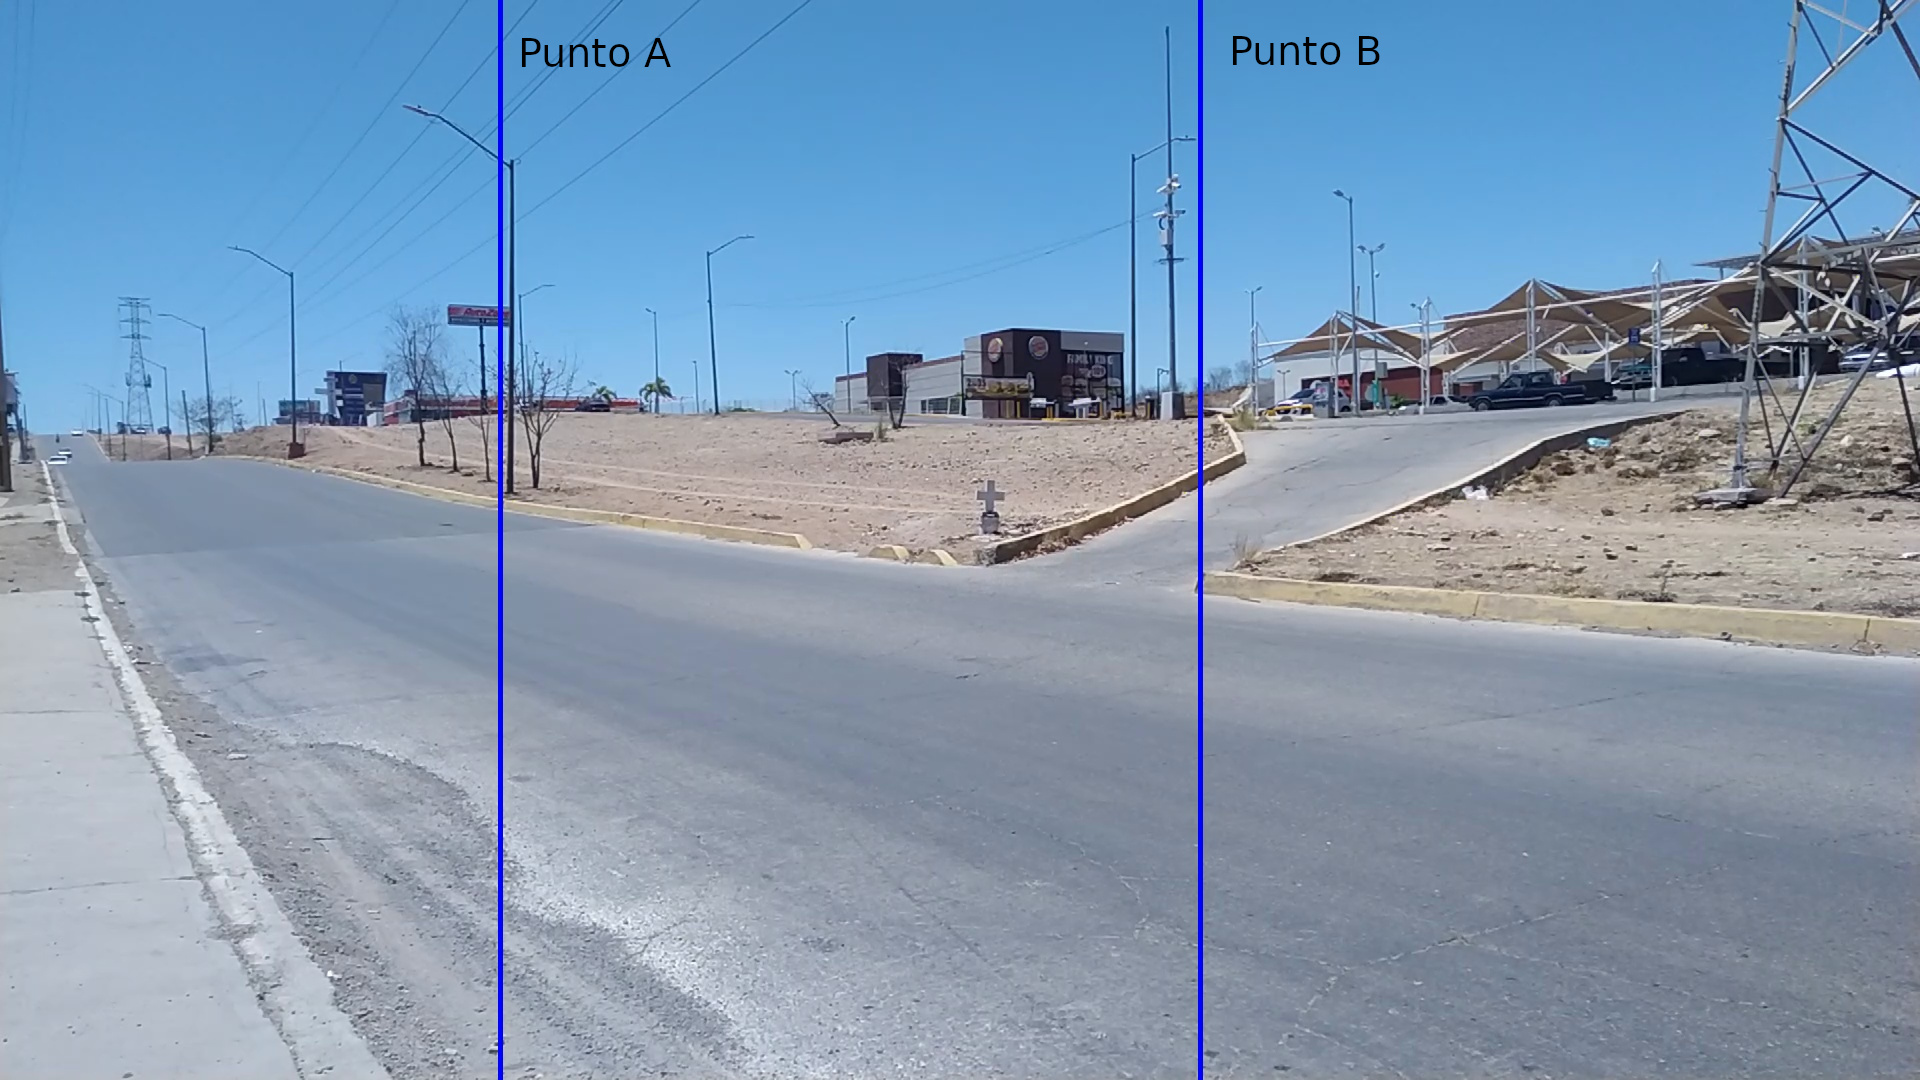
\includegraphics[width=0.8\textwidth]{Metodologia/imgs/LugarLimites_01.jpg}
    \caption{Límites para lugar de las muestras.}
    \label{fig:LugarLimites}
\end{figure}

Una vez que se deciden los valores para los puntos A y B, se genera el archivo csv. Para esto se toma en cuenta el segundo en que pasa debe ser lo más cercano posible al centroide del vehículo cuando pasa por el punto B. Es importante ingresar una descripción, aunque esta no va a ser usada por el sistema. Se volverá importante para validar que el vehículo al que se le tomó la velocidad es el mismo que detecto el sistema.

%%%%%%%%%%%%%%%%%%%%%%%%%%%%%%%%%%%%%%%%%%%%%%%%%%%%%%%%%%%%%%%%%%%%%%%%%%%%%%%%
%%%%%%%%%%%%%%%%%%%%%%%%%%%%%%%%%%%%%%%%%%%%%%%%%%%%%%%%%%%%%%%%%%%%%%%%%%%%%%%%
%%%%%%%%%%%%%%%%%%%%%%%%%%%%%%%%%%%%%%%%%%%%%%%%%%%%%%%%%%%%%%%%%%%%%%%%%%%%%%%%
%%%%%%%%%%%%%%%%%%%%%%%%%%%%%%%%%%%%%%%%%%%%%%%%%%%%%%%%%%%%%%%%%%%%%%%%%%%%%%%%
%%%%%%%%%%%%%%%%%%%%%%%%%%%%%%%%%%%%%%%%%%%%%%%%%%%%%%%%%%%%%%%%%%%%%%%%%%%%%%%%

\section{Obtención de velocidad}

Como se mencionó anteriormente en la Sección \ref{cap:metodologia} la obtención de la velocidad se divide en tres partes las cuales están representadas en el Figura \ref{fig:DFObtencionDeVelocidad} y se describen a continuación.

\begin{figure}[H]
    \centering
    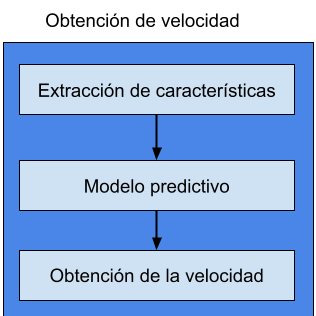
\includegraphics[width=0.5\textwidth]{Metodologia/imgs/ObtencionVelocidad.png}
    \caption{Proceso de obtención de velocidad.}
    \label{fig:DFObtencionDeVelocidad}
\end{figure}

\subsection{Extracción de características }

En el paso anterior para cada muestra se creo un archivo csv el cual servirá de entrada para el paso actual.

El sistema se encarga de leer el video utilizando la biblioteca OpenCV con la cual se extraen los fotogramas del video, cada fotograma pasa por la red neuronal YOLO la cual se encarga de identificar todos los vehículos que aparecen en el fotograma. YOLO regresa las coordenadas de cada objeto detectado dentro del fotograma, estas coordenadas son usadas para dibujar un recuadro para cada objeto. La Figura \ref{fig:LugarDeteccion} muestra dos vehículos detectados.

\begin{figure}[H]
    \centering
    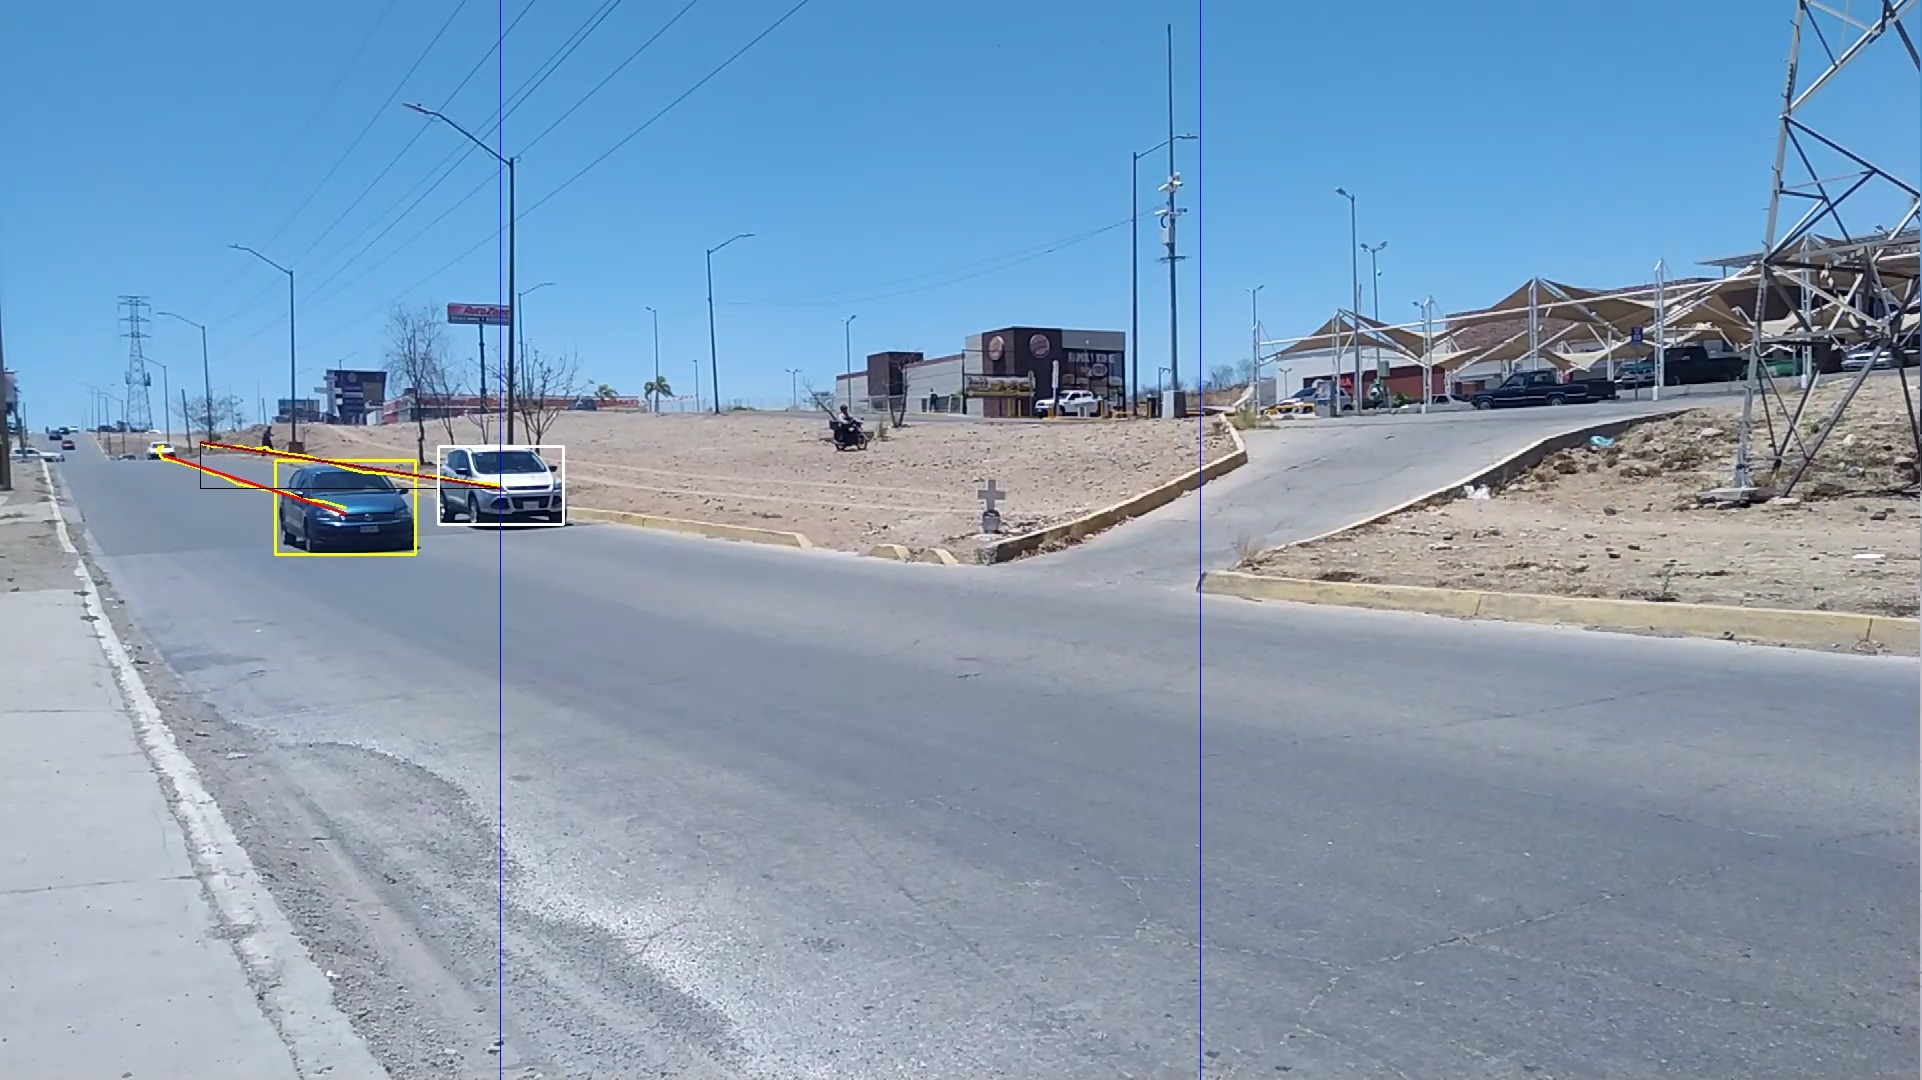
\includegraphics[width=0.8\textwidth]{Metodologia/imgs/Deteccion.jpg}
    \caption{Detección de vehículos dentro de recuadros.}
    \label{fig:LugarDeteccion}
\end{figure}

El seguimiento de los vehículos se realiza por medio del Filtro Kalman el cual determina su ubicación en el próximo fotograma. El sistema se encarga de guardar todas las ubicaciones de los vehículos en el transcurso del tiempo siendo capaz dibujar todo el trayecto que han tenido cada uno de ellos. Sumando el uso de regresión lineal se crea una recta que corresponde a las trayectorias de los vehículos. La Figura \ref{fig:LugarSeguimiento} muestra un vehículo detectado en un recuadro blanco, una línea amarilla con la trayectoria del vehículo y una línea roja la cual es generada con regresión a partir de la trayectoria del vehículo.

\begin{figure}[H]
    \centering
    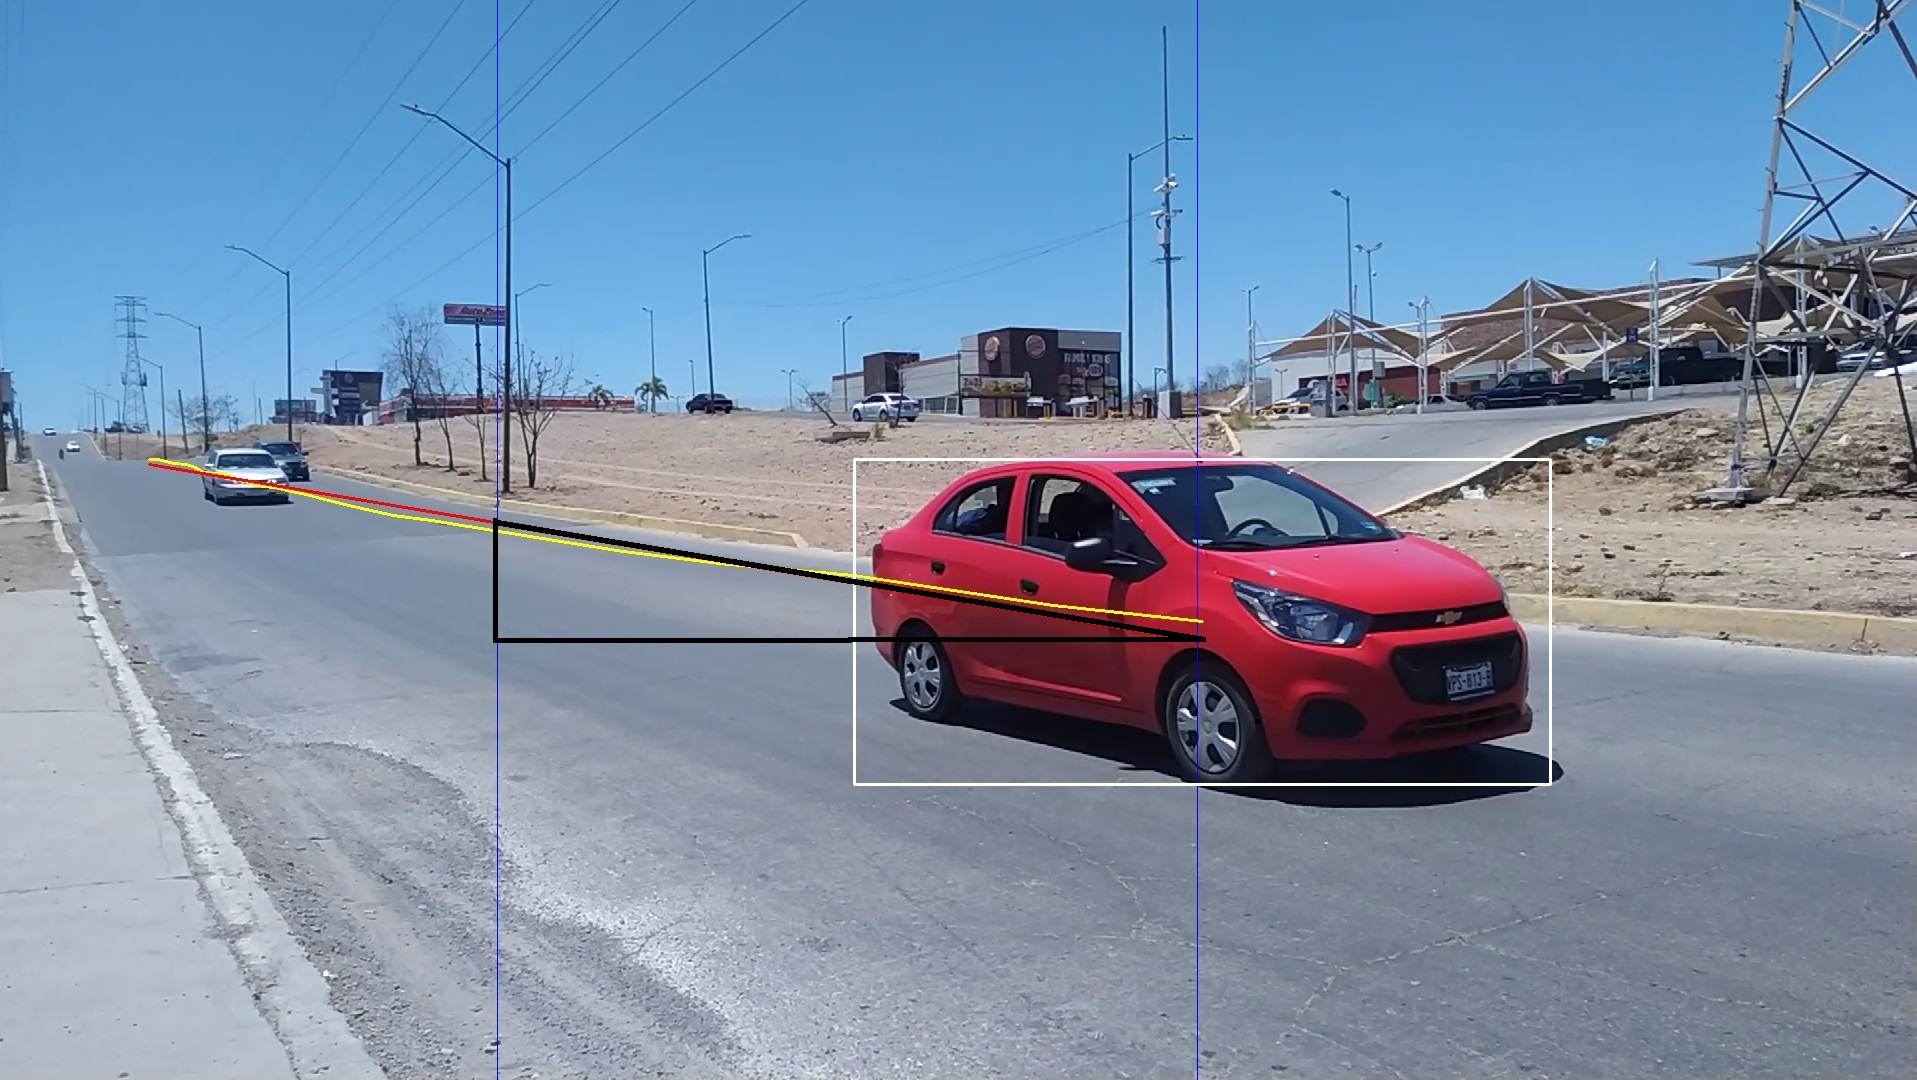
\includegraphics[width=0.8\textwidth]{Metodologia/imgs/Seguimiento_01.jpg}
    \caption{Detección de vehículos en punto B, sus trayectorias y triangulación del generado con el punto A y B.}
    \label{fig:LugarSeguimiento}
\end{figure}

Otra característica que se identifica en la Figura \ref{fig:LugarSeguimiento} es la creación de un triángulo en color negro, con el cual se identifica el ángulo detectado para el vehículo.

Cando el sistema detecta que un vehículo pasa por el punto A, este guarda la información del estado del vehículo (Figura \ref{fig:PuntoA}). Puede haber múltiples vehículos pasando en ese momento y todos serán detectados por el sistema. El vehículo del cual se obtienen sus características esta identificado con un recuadro de color amarillo, mientras que el resto de los vehículos están dentro de un recuadro color amarillo.


\begin{figure}[H]
    \centering
    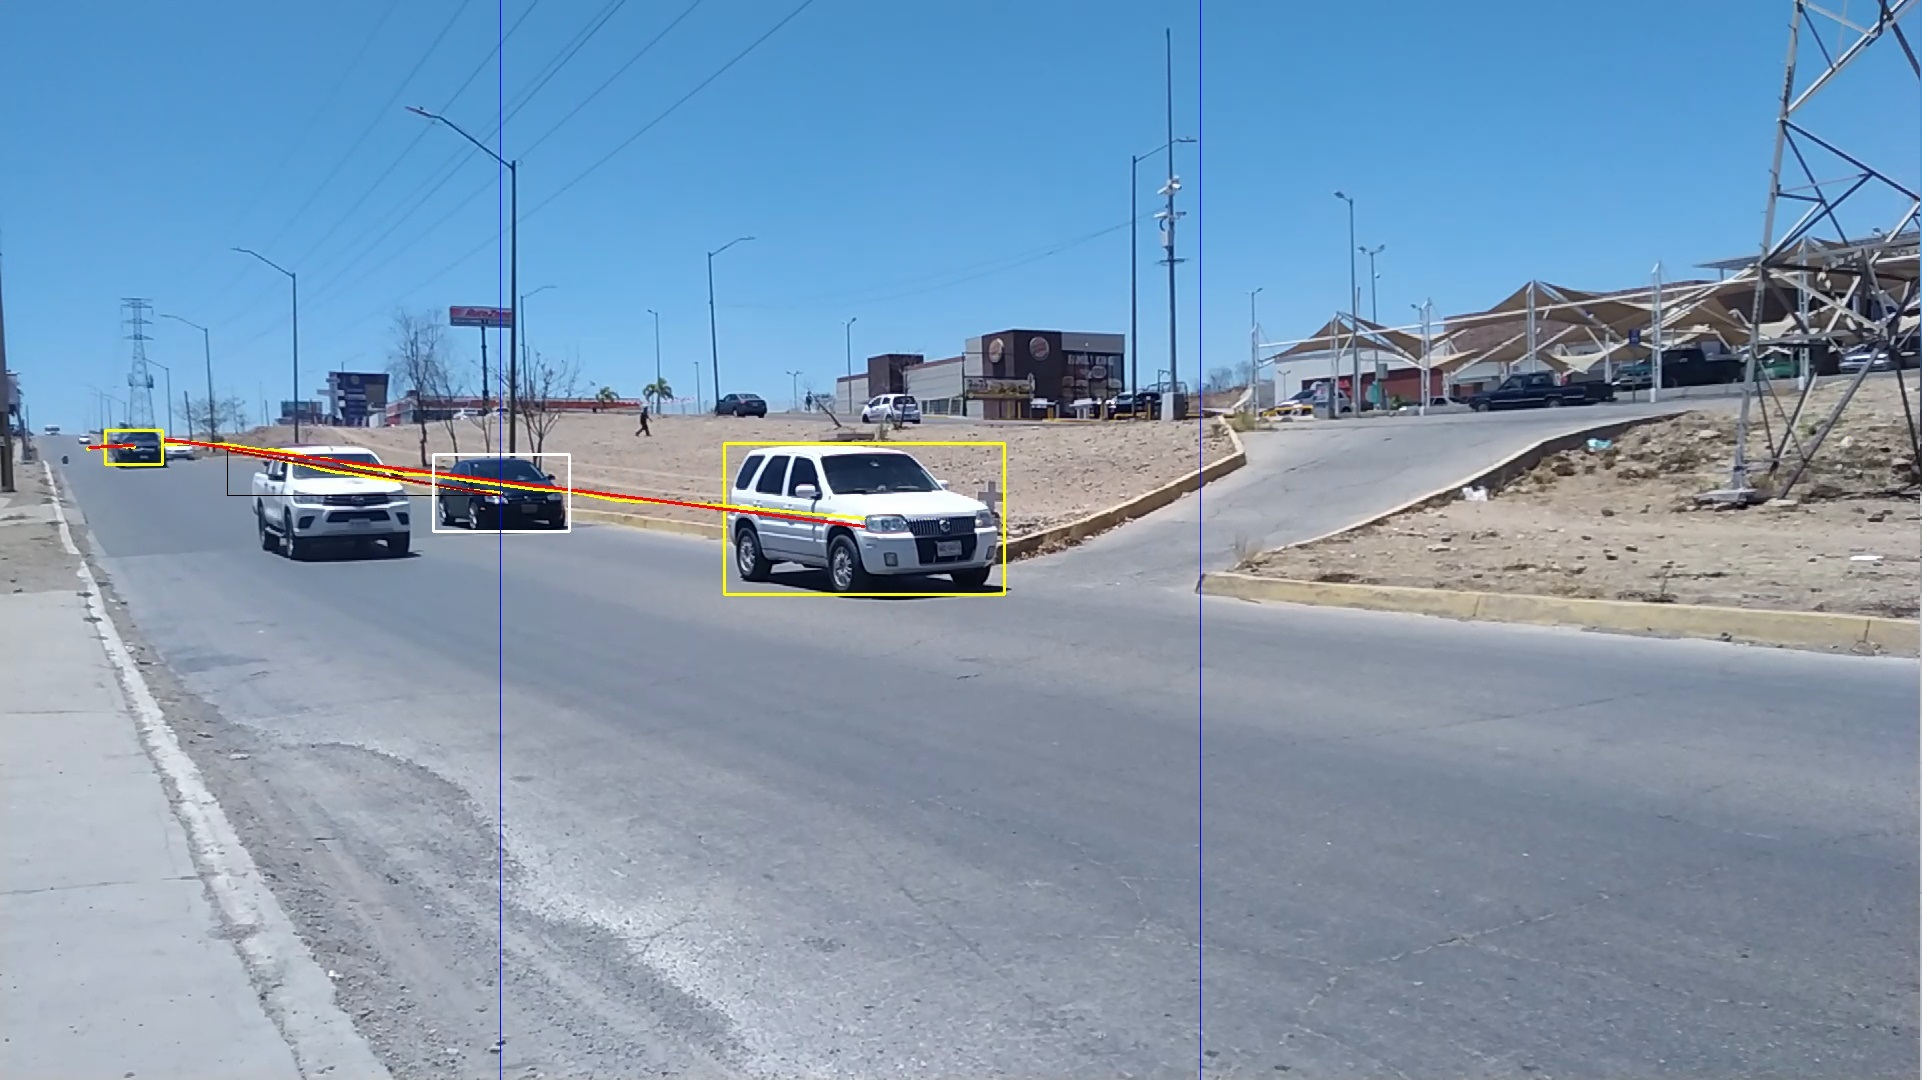
\includegraphics[width=0.8\textwidth]{Metodologia/imgs/Punto_A.jpg}
    \caption{Punto A con vehículo en recuadro blanco.}
    \label{fig:PuntoA}
\end{figure}

Aunque se guardó el estado del vehículo cuando paso por el punto A, este no genera una línea para el archivo csv resultante. Es hasta que el vehículo pasa por el punto B y coincide con los segundos en el archivo csv de entrada que el sistema guarda un nuevo dato en el archivo de salida. Los vehículos que no cuentan con una línea en el archivo csv de entrada no se les guarda su información. La Figura \ref{fig:PuntoB} muestra cuando el vehículo detectado en el punto A pasa por el punto B.

\begin{figure}[H]
    \centering
    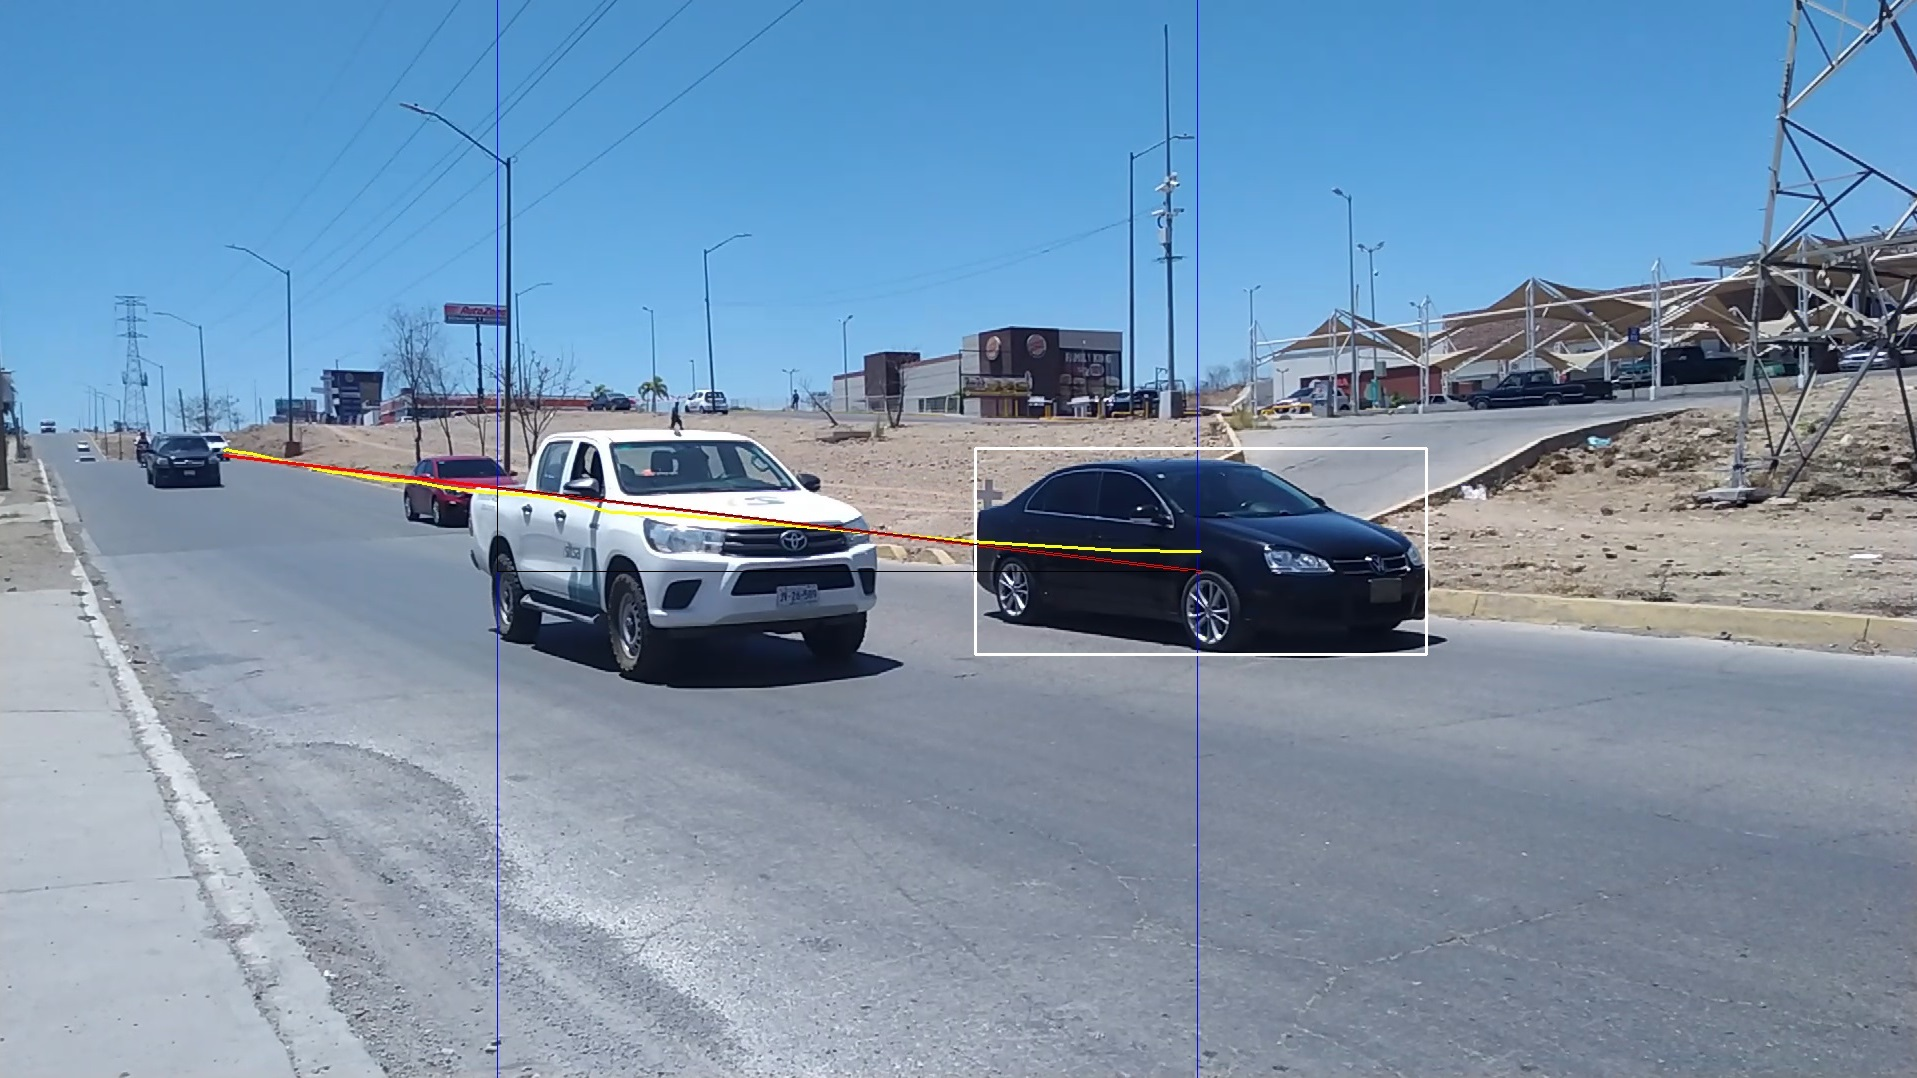
\includegraphics[width=0.8\textwidth]{Metodologia/imgs/Punto_B.jpg}
    \caption{Punto B con vehículo en recuadro blanco.}
    \label{fig:PuntoB}
\end{figure}

La Tabla \ref{tab:CaracteristicasSistema} muestra las características más importante que son extraídas por el sistema y una descripción.

\begin{table}[H]
    \caption{Características obtenidas por el sistema.}
    \label{tab:CaracteristicasSistema}
    \begin{tabular}{|l|l|}
        \hline
        \textbf{Característica} & \multicolumn{1}{c|}{\textbf{Descripción}} \\ \hline
        \textbf{Ángulo Salida} & Ángulo a partir del punto de entrada hasta el punto de salida \\ \hline
        \textbf{Distancia de salida} & Distancia recorrida desde el punto de entrada hasta el punto de salida \\ \hline
        \textbf{Área Entrada} & Área detectada del vehículo en pixeles en el punto de entrada \\ \hline
        \textbf{Área Salida} & Área detectada del vehículo en pixeles en el punto de salida \\ \hline
        \textbf{FPS} & Fotogramas por segundo del video \\ \hline
        \textbf{Tiempo} & Tiempo que le tomo al vehículo para pasar del punto entrada al de salida \\ \hline
        \textbf{Velocidad} & Velocidad detectada por el radar \\ \hline
        \textbf{Carril} & Carril por que pasa el vehículo \\ \hline
        \textbf{Identificador} & Identificador correspondiente a una imagen generada \\ \hline
    \end{tabular}
\end{table}


El sistema además de generar un archivo csv, crea una imagen de salida la cual corresponde a una línea del archivo resultante, esta imagen está formada por dos imágenes una al lado de la otra, la imagen de la izquierda representa el vehículo cuando entra en el punto A y la imagen de la derecha es cuando el vehículo pasa por el punto B. La Figura \ref{fig:Completo} muestra un ejemplo de esta imagen de salida.

\begin{figure}[H]
    \centering
    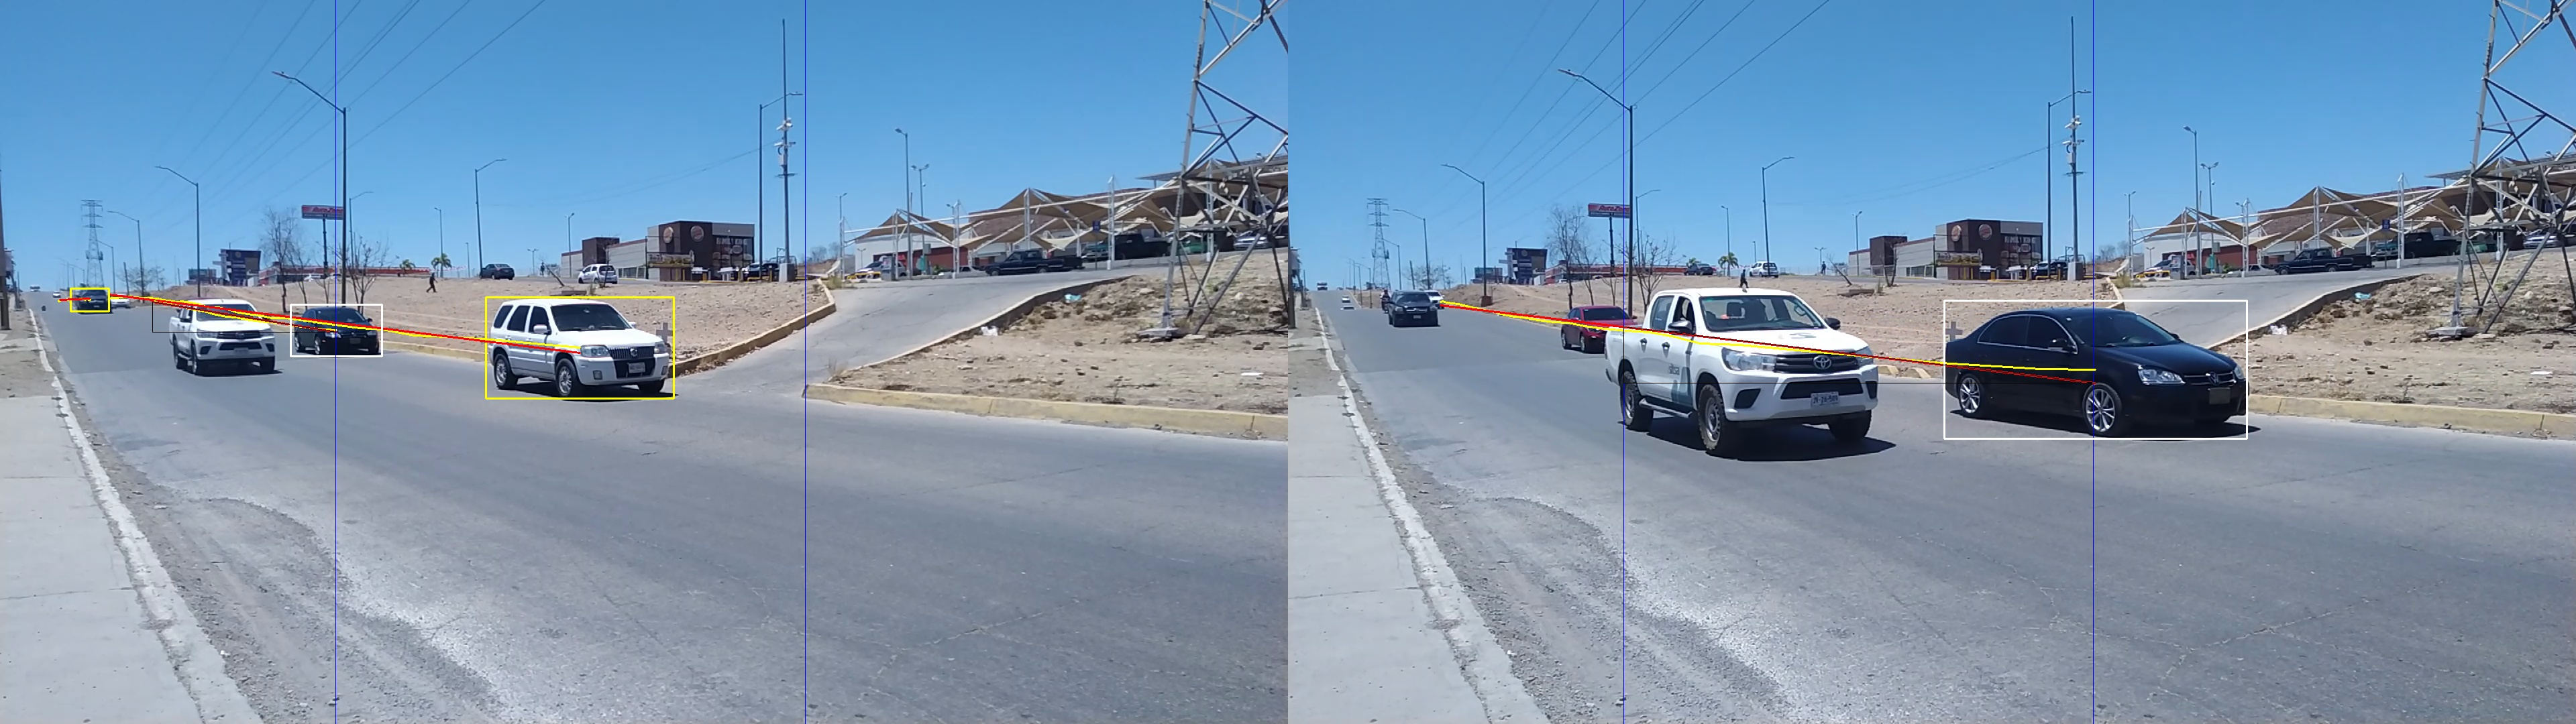
\includegraphics[width=1\textwidth]{Metodologia/imgs/Completo.jpg}
    \caption{Imagen resultado para cada línea de archivo csv.}
    \label{fig:Completo}
\end{figure}

%%%%%%%%%%%%%%%%%%%%%%%%%%%%%%%%%%%%%%%%%%%%%%%%%%%%%%%%%%%%%%%%%%%%%%%%%%%%%%%%
%%%%%%%%%%%%%%%%%%%%%%%%%%%%%%%%%%%%%%%%%%%%%%%%%%%%%%%%%%%%%%%%%%%%%%%%%%%%%%%%
%%%%%%%%%%%%%%%%%%%%%%%%%%%%%%%%%%%%%%%%%%%%%%%%%%%%%%%%%%%%%%%%%%%%%%%%%%%%%%%%
%%%%%%%%%%%%%%%%%%%%%%%%%%%%%%%%%%%%%%%%%%%%%%%%%%%%%%%%%%%%%%%%%%%%%%%%%%%%%%%%
%%%%%%%%%%%%%%%%%%%%%%%%%%%%%%%%%%%%%%%%%%%%%%%%%%%%%%%%%%%%%%%%%%%%%%%%%%%%%%%%

Una vez que el sistema genera las imágenes de salida. El archivo csv resultante valida que el vehículo detectado sea el correcto y que el recuadro blanco que define la detección del vehículo contenga la mayor parte del vehículo.

Para el caso de validar que el vehículo sea el correcto, es necesario ver cada una de las imágenes generadas y leer la descripción en el archivo csv de entrada. En caso de identificar un vehículo que no corresponda, se debe modificar los segundos en el archivo csv de entrada de tal manera que el sistema detecte el vehículo  correcto, esto implica ejecutar el sistema nuevamente para generar los datos de nuevo. 

Existen dos casos en los que el sistema no podrá identificar el vehículo. El primer caso implica que el vehículo sea obstaculizado por otro. Por lo cual, la detección será del vehículo que esta frente al vehículo que se le esta realizando el seguimiento. El segundo caso corresponde cuando al vehículo no se le realizo el seguimiento completo del punto A al B de forma correcta, esto implica que el vehículo no fue detectado en el camino. Para estos dos caso se elimina la línea correspondiente en el archivo de entrada, lo cual también implica ejecutar el sistema nuevamente para generar los datos nuevamente.


Para validar que el área de detección del vehículo sea completa, se realizó una inspección visual de las imágenes generadas. Durante la inspección se identifica
el vehículo cuando entra en el punto A (Figura \ref{fig:ImagenValida01}) el cual debe ser detectado completamente por el recuadro blanco, al mismo tiempo que se identifica el vehículo cuando pasa por el punto B (Figura \ref{fig:ImagenValida02}) el cual también debe ser identificado completamente por el recuadro blanco.


\begin{figure}[H]
    \centering
    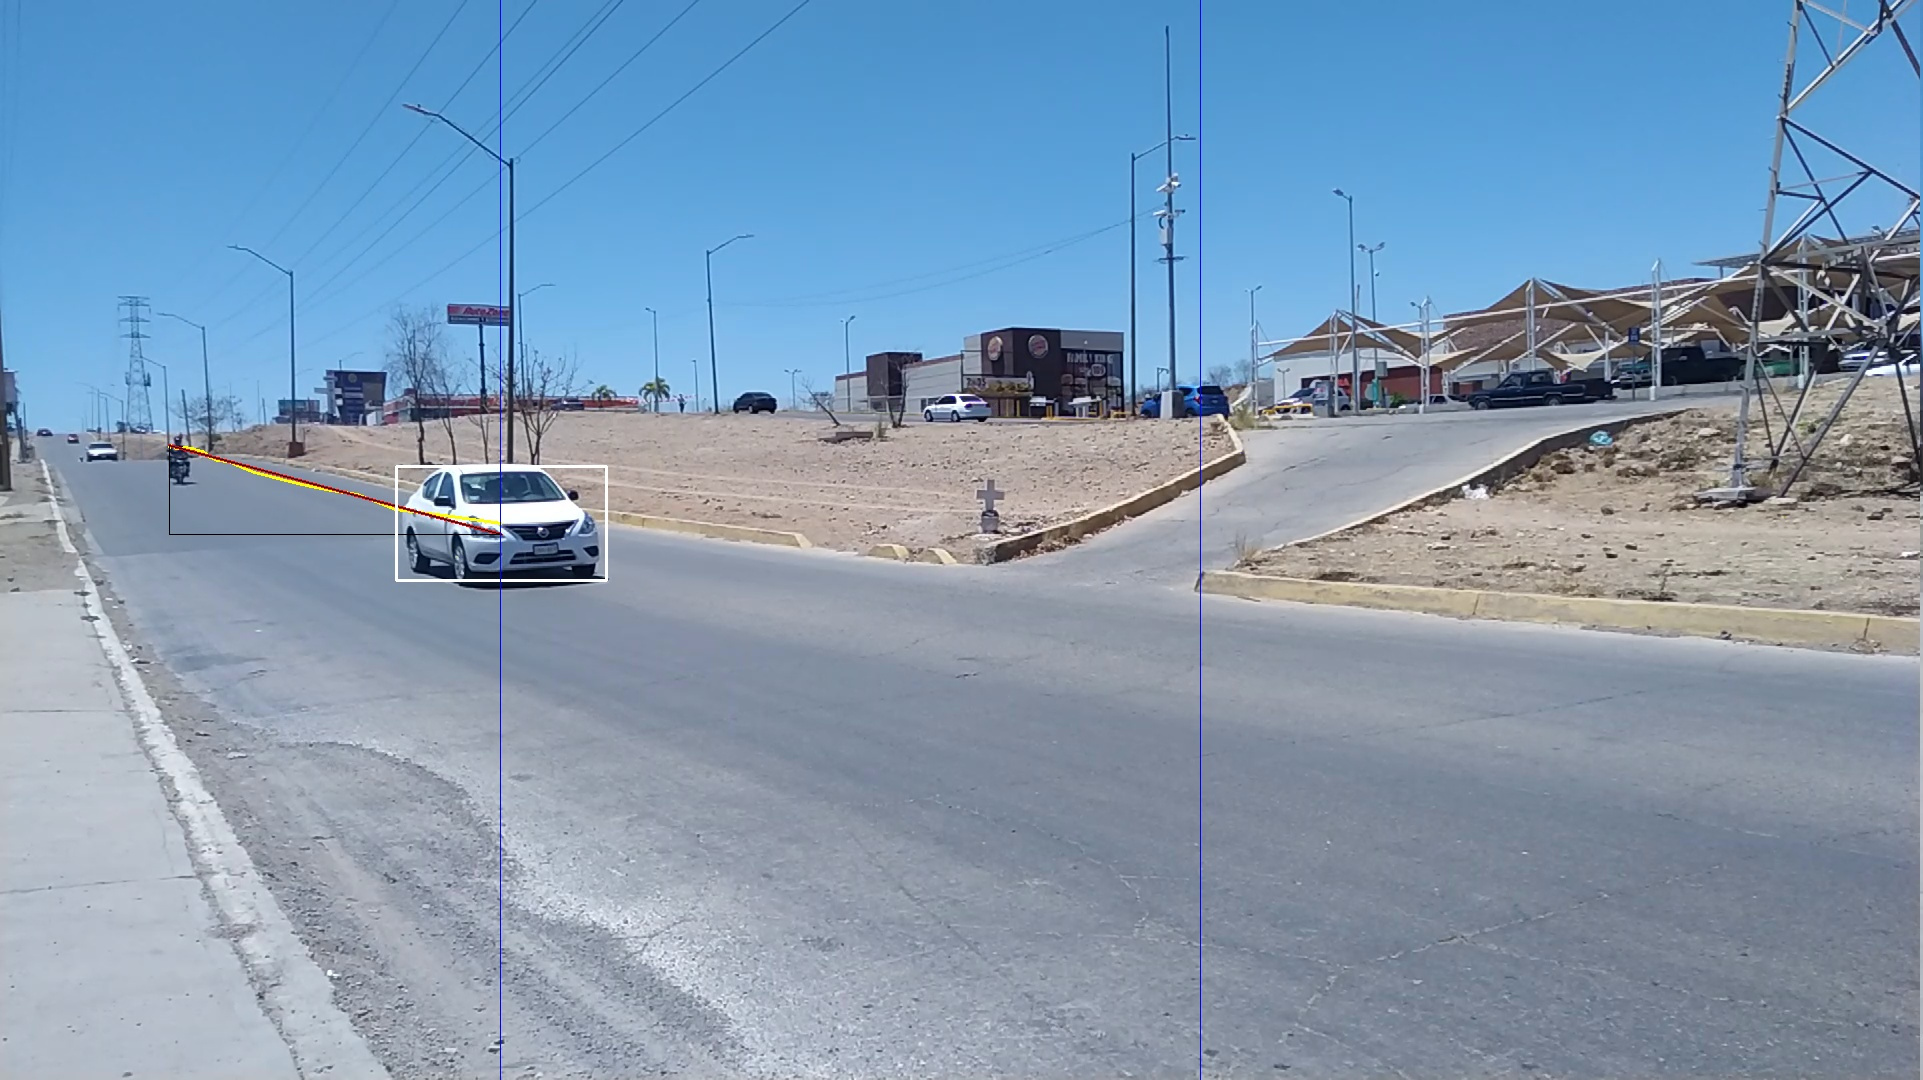
\includegraphics[width=0.8\textwidth]{Metodologia/imgs/Valido_001.jpg}
    \caption{Imagen válida con vehículo entrando representando una línea del archivo csv.}
    \label{fig:ImagenValida01}
\end{figure}

\begin{figure}[H]
    \centering
    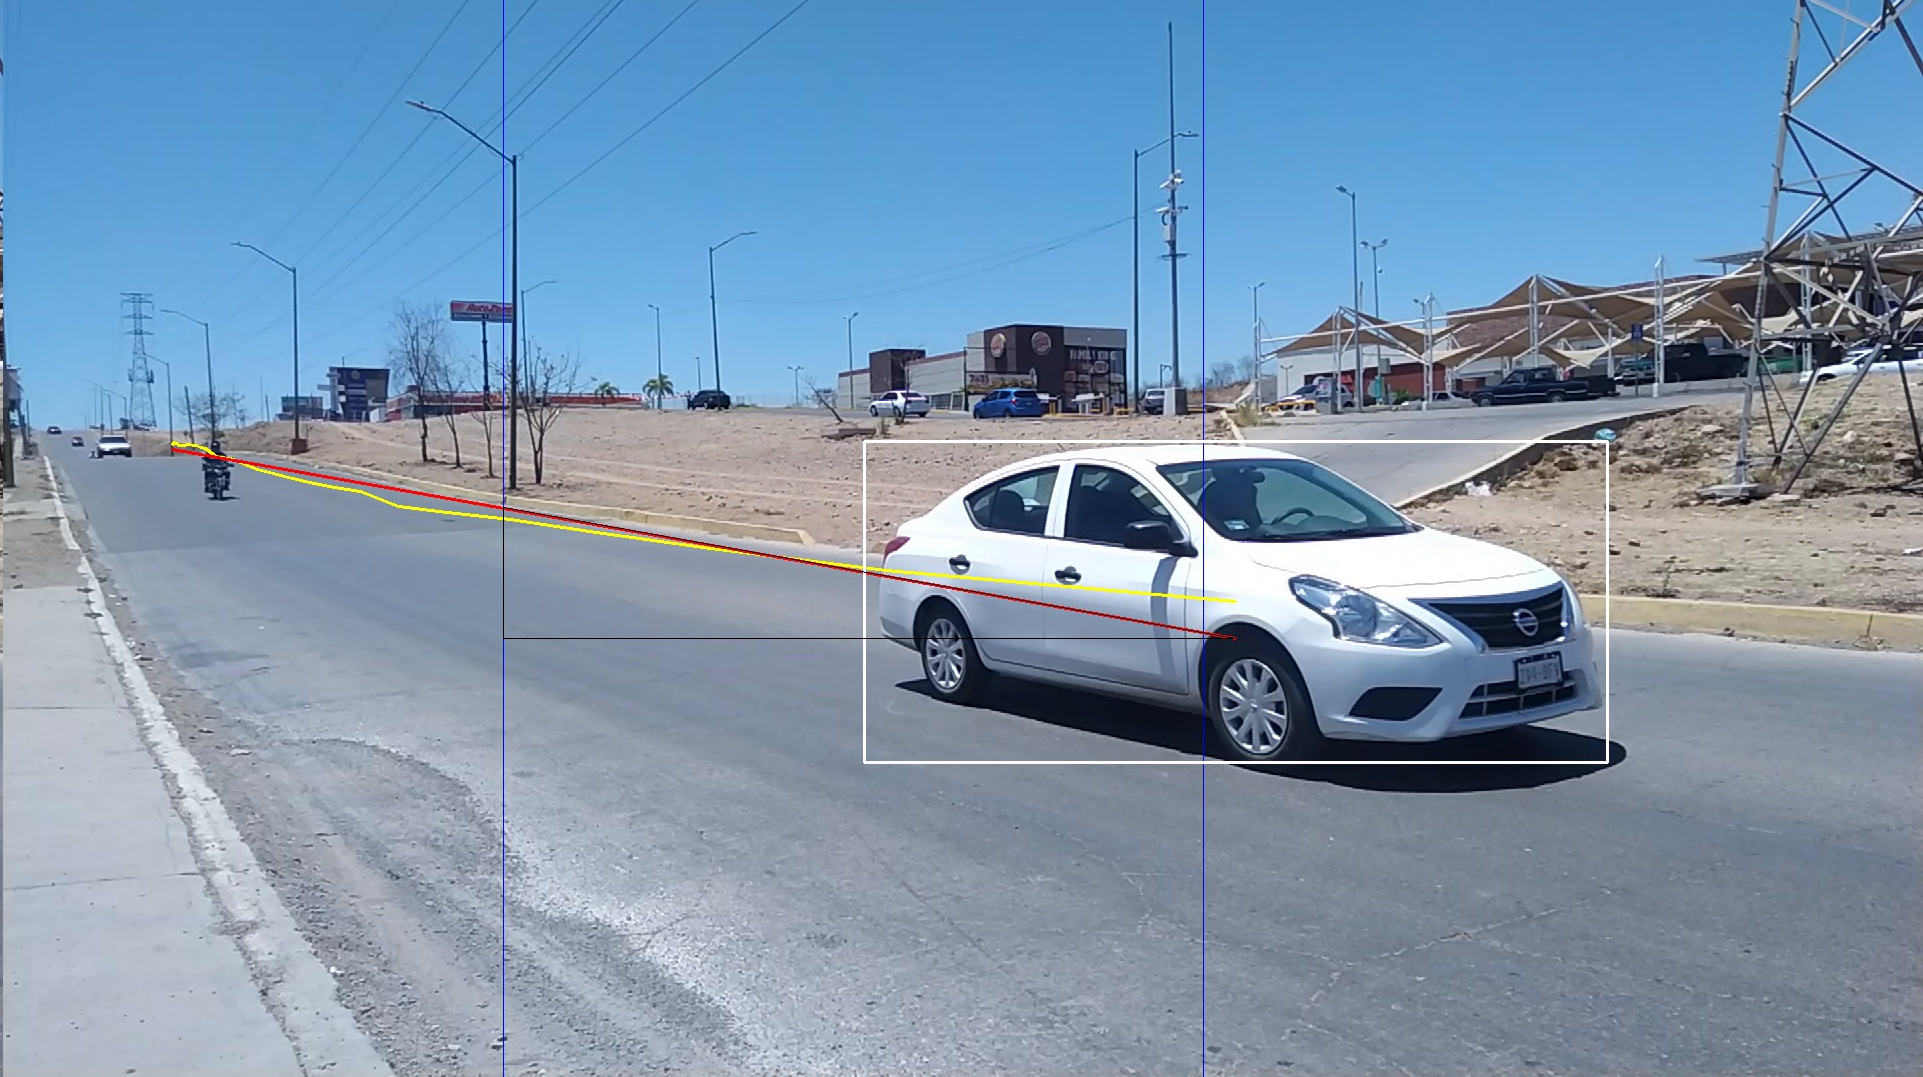
\includegraphics[width=0.8\textwidth]{Metodologia/imgs/Valido_002.jpg}
    \caption{Imagen válida con vehículo saliendo representando una línea del archivo csv.}
    \label{fig:ImagenValida02}
\end{figure}

Por otra parte, hay ocasiones en la cuales el sistema solo detecta parte del vehículo. En este caso la muestra se considera como inválida. Un ejemplo, la Figura \ref{fig:ImagenInvalida_01} muestra el vehículo detectado completamente en el punto A, mientras que cuando el vehículo sale por el punto B es detectado solo una parte (Figura \ref{fig:ImagenInvalida_02}).

\begin{figure}[H]
    \centering
    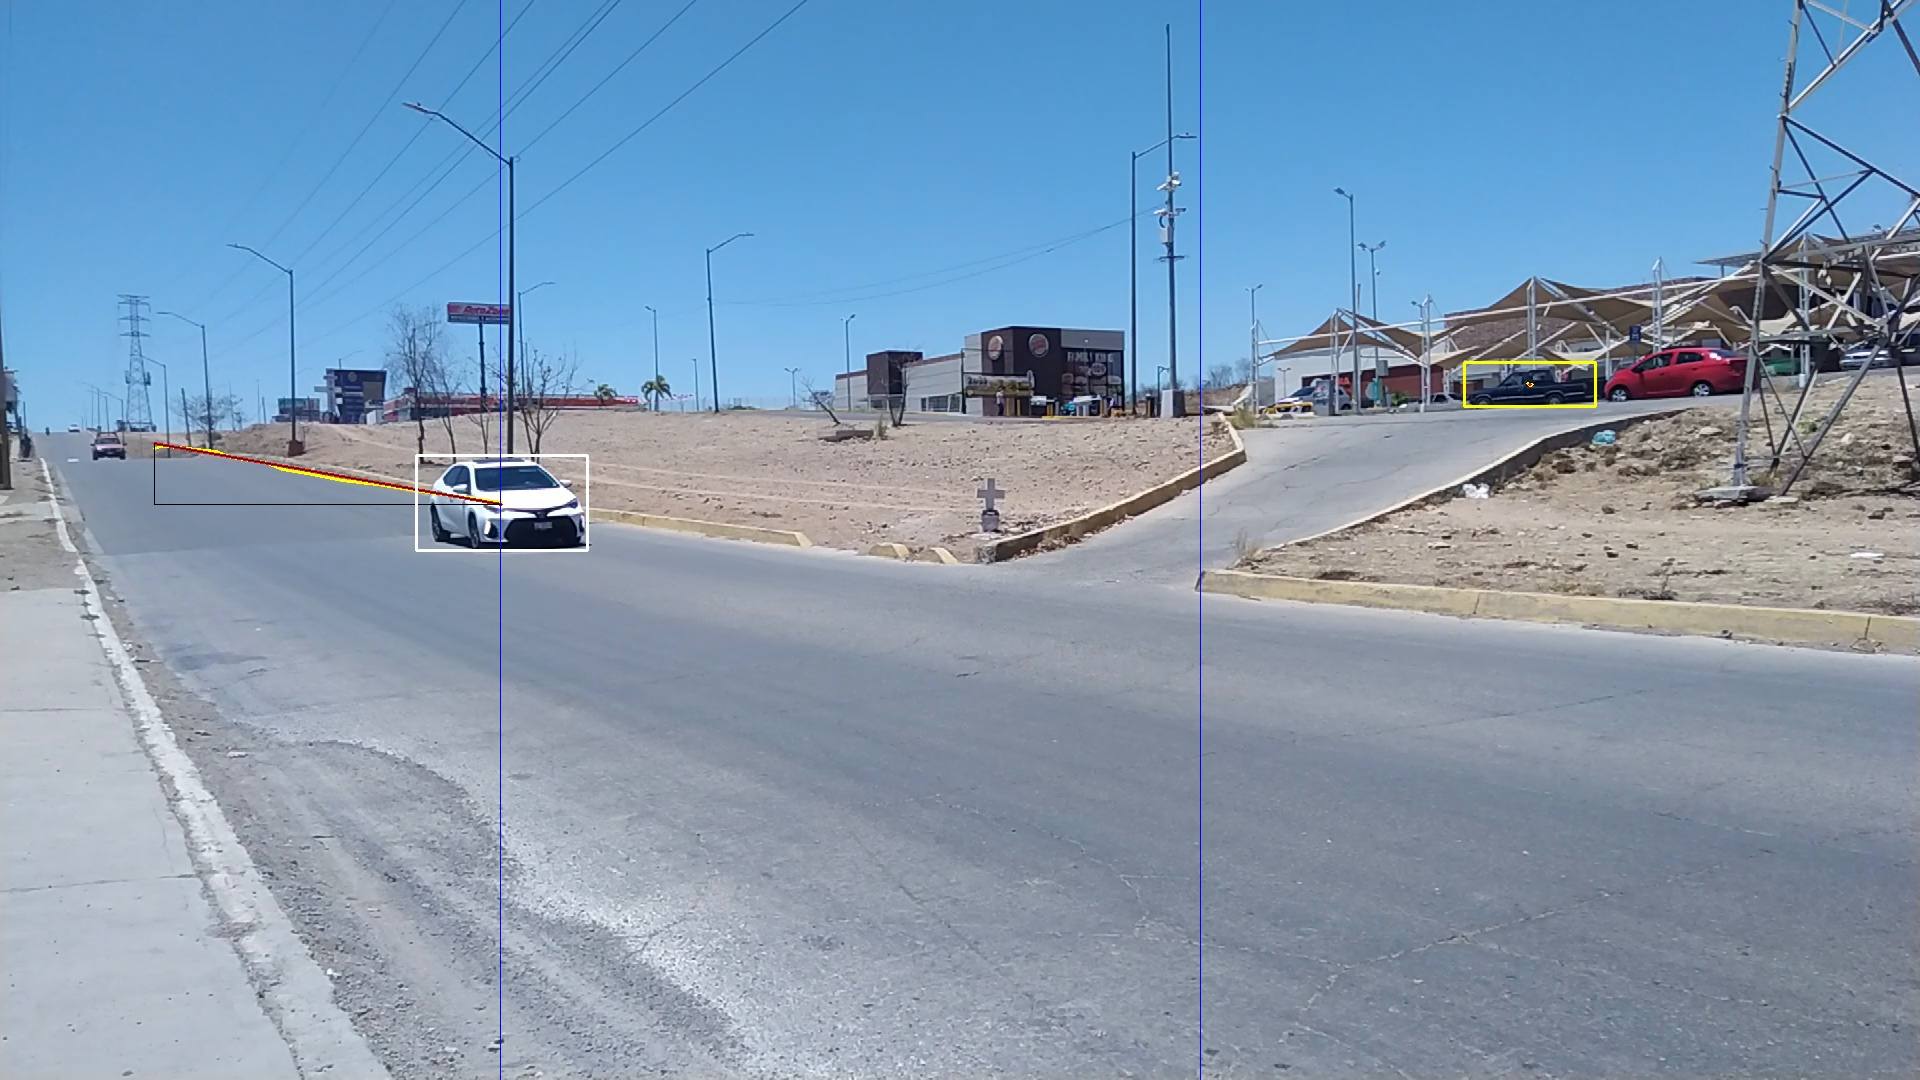
\includegraphics[width=0.8\textwidth]{Metodologia/imgs/Invalido_001.jpg}
    \caption{Imagen inválida (parte izquierda) con vehículo entrando representando una línea del archivo csv.}
    \label{fig:ImagenInvalida_01}
\end{figure}

\begin{figure}[H]
    \centering
    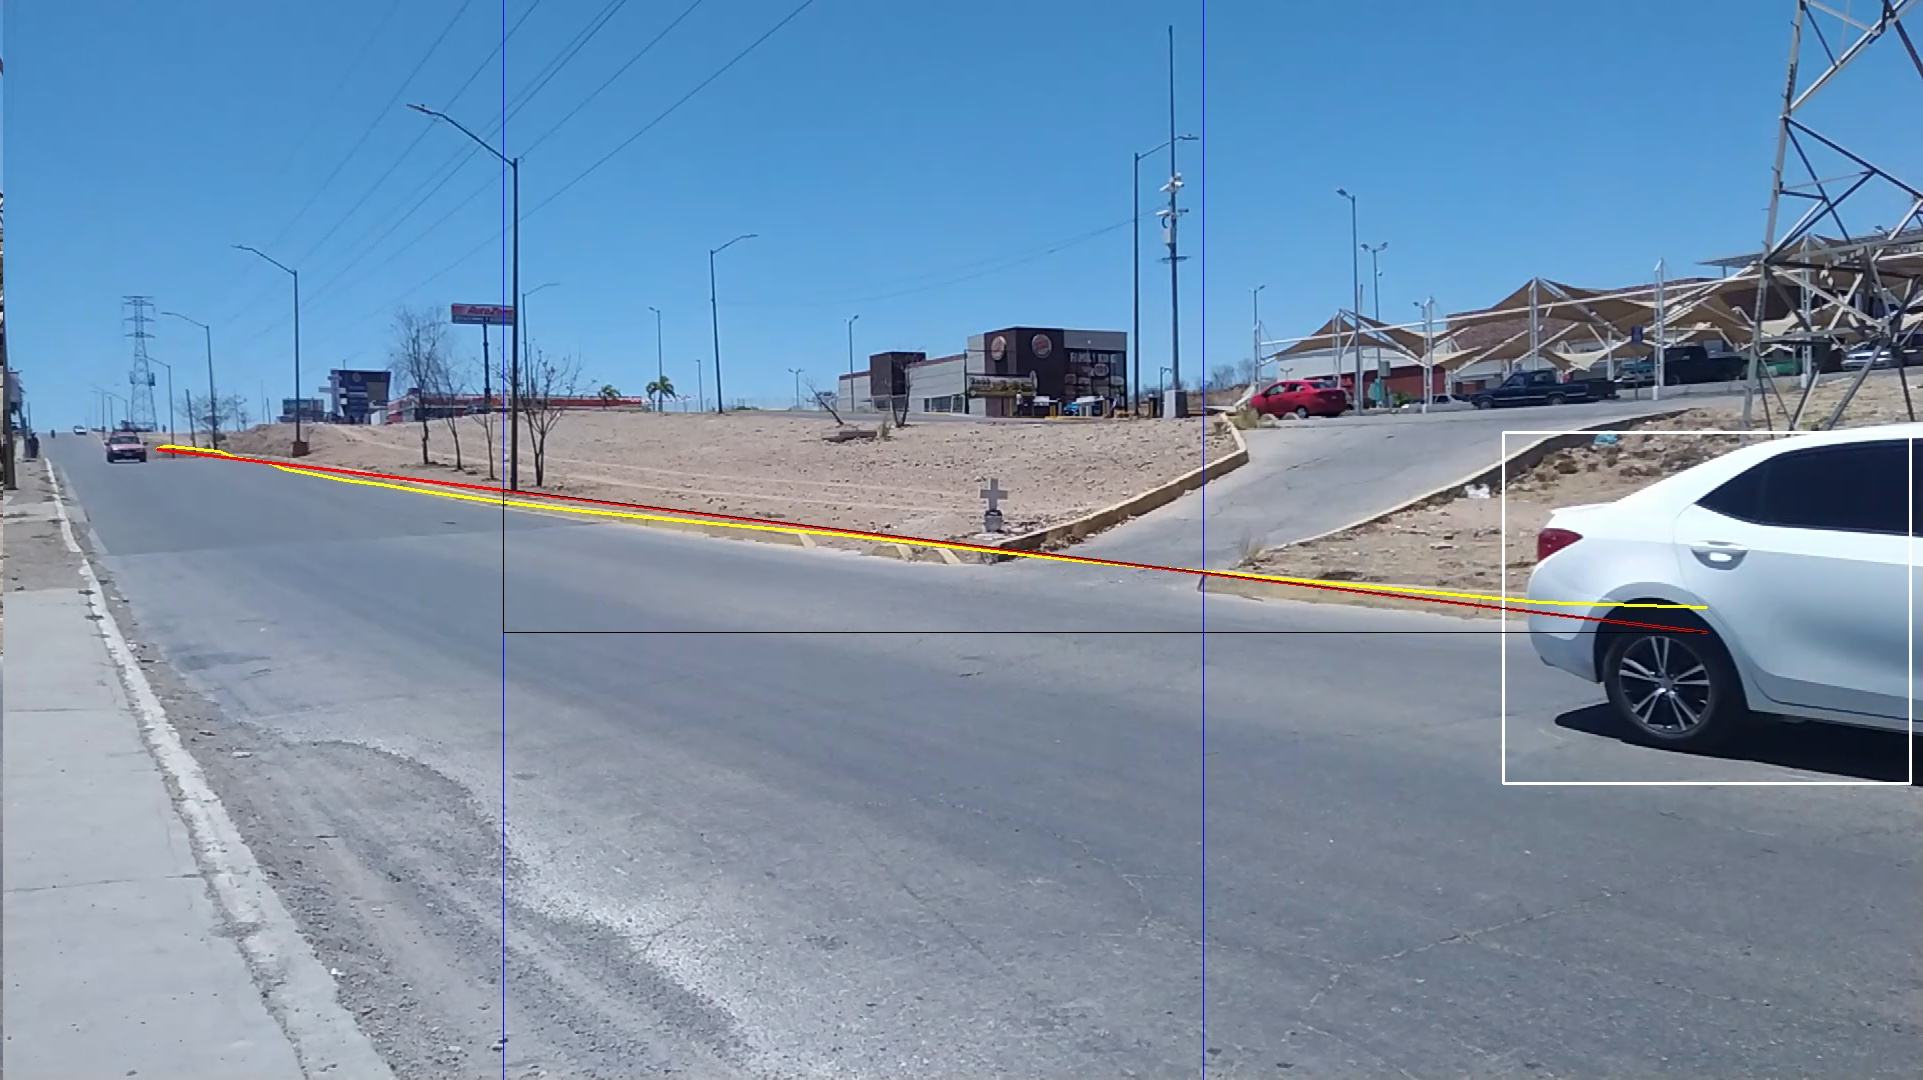
\includegraphics[width=0.8\textwidth]{Metodologia/imgs/Invalido_002.jpg}
    \caption{Imagen inválida (parte derecha) con vehículo saliendo representando una línea del archivo csv.}
    \label{fig:ImagenInvalida_02}
\end{figure}

Una vez que se identifica una imagen inválida se elimina la muestra correspondiente en el archivo csv de salida. Esta muestra se reconoce por el identificador descrito en la Tabla \ref{tab:CaracteristicasSistema}. Para este caso no es necesario volver a ejecutar el sistema.


\subsection{Modelo predictivo}
\label{cap:EstimacionVelocidad}

En esta sección se describe la metodología utilizada para crear un proceso o modelo el cual podamos utilizar para determinar la velocidad de vehículos, se implementaron dos metodologías para esta tarea, el primero utiliza la fórmula física de la velocidad, a partir de esta fórmula se busca un factor de correlación entre la distancia en pixeles recorrida por el vehículo y la distancia real, mientras que el segundo método implementado es el entrenamiento de un modelo de aprendizaje máquina utilizando bibliotecas de Python las cuales nos ayudan a crear un modelo con el cual podemos determinar la velocidad.

\subsubsection{Estimar velocidad basado en factor de correlación}

Para determinar la velocidad utilizando el conjunto de datos generado por el sistema se inicia a partir de lo más sencillo utilizando la fórmula física para el cálculo de la velocidad, Ecuación \ref{eq:Velocidad}.

\begin{equation}
    \label{eq:Velocidad}
    Velocidad = \frac{Distancia}{Tiempo}
\end{equation}

En este caso las muestras fueron tomadas por un Radar que solo nos proporciona la velocidad en Kilómetros o en Millas, así que necesitamos convertir este valor a Metros sobre segundo, utilizando la Ecuación \ref{eq:ConvertMSKH}.

\begin{equation}
    \label{eq:ConvertMSKH}
    \frac{M}{S} = \frac{18}{5} \times \frac{K}{H}
\end{equation}

A partir de la formula física para el cálculo de la velocidad y la conversión de la velocidad en metros por segundo en lugar de kilómetros por hora, podemos definir el proceso para crear el modelo en el diagrama de flujo que se muestra en la Figura \ref{fig:CrearModeloCustom}.

\begin{figure}[H]
    \centering
    \begin{tikzpicture}
        \node(a)[circle, draw=black, minimum size=1.5cm]
            {Inicio};

        \node(b)[rectangle, draw=black, minimum width=5cm, minimum height=1.7cm]
            [right=of a]
            [text width=5cm, align=center]
            {Calcular distancia estimada};
        \node(c)[rectangle, draw=black, minimum width=5cm, minimum height=1.7cm]
            [right=of b]
            [text width=5cm, align=center]
            {Encontrar factor de correlación};
        \node(d)[rectangle, draw=black, minimum width=5cm, minimum height=1.7cm]
            [below=of c]
            [text width=5cm, align=center]
            {Promediar factor de correlación};
        \node(e)[rectangle, draw=black, minimum width=5cm, minimum height=1.7cm]
            [left=of d]
            [text width=5cm, align=center]
            {Integrar factor de correlación con formula de velocidad};

        \node(f)[circle, draw=black, minimum size=1.5cm]
            [left=of e]
            {Fin};

        \draw[->] (a) -- (b);
        \draw[->] (b) -- (c);

        \draw[->] (c) -- (d);
        \draw[->] (d) -- (e);
        \draw[->] (e) -- (f);


    \end{tikzpicture}

    \caption{Diagrama de flujo para la creación de modelo con la formula física de la velocidad.}
    \label{fig:CrearModeloCustom}
\end{figure}

La Tabla \ref{tab:CaracteristicasSistema} muestra que los tres parámetros necesarios para estimar la velocidad, sin embargo, el valor de la distancia está en pixeles, por lo que es necesario convertir el valor a una distancia estimada, este valor es convertido con la Ecuación \ref{eq:Velocidad} despejando la distancia, con esto se obtiene la  Ecuación \ref{eq:DistanciaEstimada}.

\begin{equation}
    \label{eq:DistanciaEstimada}
    Distancia\:Estimada = Tiempo \times Velocidad
\end{equation}

Una vez que se tiene la distancia estimada, debemos encontrar la correlación entre esta y la distancia en pixeles, con lo cual tenemos la siguiente Ecuación \ref{eq:EcuacionB}.

\begin{equation}
    \label{eq:EcuacionB}
    B = \frac{Distancia \: Estimada}{Distancia \: Pixeles}
\end{equation}

A este valor lo llamamos simplemente B, el valor de B es utilizado para calcular una velocidad estimada con respecto a la distancia y el tiempo, lo cual quedaría como muestra la Ecuación \ref{eq:VelocidadB}.

\begin{equation}
    \label{eq:VelocidadB}
    Velocidad = \frac{Distancia \: Pixeles}{Tiempo} \times B
\end{equation}

Sin embargo, esta fórmula solo servirá para un dato en específico generado por el sistema por lo cual debemos encontrar un valor de B que modele la gran mayoría de nuestras muestras o tener un error lo más bajo posible, para esto se calcula el valor de B para todas las muestras y se calcula el promedio de B, Ecuación \ref{eq:PromedioB}.

\begin{equation}
    \label{eq:PromedioB}
    \overline{B} = \frac{\sum B}{n}
\end{equation}

Una vez se tiene B promedio se puede sustituir por B en la Ecuación \ref{eq:VelocidadB} lo cual quedaría como muestra la Ecuación \ref{eq:VelocidadBPromedio}.

\begin{equation}
    \label{eq:VelocidadBPromedio}
    Velocidad = \frac{Distancia \: Pixeles}{Tiempo} \times \overline{B}
\end{equation}



\subsubsection{Estimar velocidad Scikit y Tensor Flow}

El proceso de creación del modelo de Scikit y Tensor Flow son el mismo, este se describe en el diagrama de flujo de la Figura \label{ref:ModeloScikitTensorFlow}.

\begin{figure}[H]
    \centering
    \begin{tikzpicture}[node distance=5mm]

        \node(a)[circle, draw=black, minimum size=1cm]
            {Inicio};

        \node(b)[rectangle, draw=black, minimum width=3cm, minimum height=1.2cm]
            [right=of a]
            [text width=3cm, align=center]
            {Separar conjunto de datos};
        \node(c)[rectangle, draw=black, minimum width=3cm, minimum height=1.2cm]
            [right=of b]
            [text width=3cm, align=center]
            {Entrenar modelo};
        \node(d)[rectangle, draw=black, minimum width=3cm, minimum height=1.2cm]
            [right=of c]
            [text width=3cm, align=center]
            {Validar modelo};


        \node(e)[circle, draw=black, minimum size=1cm]
            [right=of d]
            {Fin};

        \draw[->] (a) -- (b);
        \draw[->] (b) -- (c);
        \draw[->] (c) -- (d);
        \draw[->] (d) -- (e);
    \end{tikzpicture}
    \caption{Diagrama de flujo para estimar velocidad utilizando inteligencia artificial.}
    \label{fig:ModeloScikitTensorFlow}
\end{figure}


El proceso para entrenar un modelo tanto en Scikit como Tensor Flow es el proceso más común utilizado. El primer paso es separar el conjunto de datos en un conjunto de entrenamiento y otro de validación normalmente esto se realiza en un porcentaje de 70\% - 30\%. Una vez separado el conjunto de datos se procede al entrenamiento utilizando la herramienta elegida, hasta que se tiene una precisión tan buena como se requiera. Por último, se utiliza el modelo con el conjunto de validación para garantizar que los resultados obtenidos sean tan buenos como en el conjunto de entrenamiento.


\subsection{Obtención de la velocidad}

Utilizando el conjunto de datos creado por el sistema para generar el modelo que se propone en la Sección \ref{cap:EstimacionVelocidad} podemos determinar la velocidad simplemente adquiriendo los datos de la distancia en pixeles y el tiempo más nuestra B promedio, con esto es solo cuestión de sustituir los valores en la Ecuación \ref{eq:VelocidadBPromedio}.

Por ejemplo, calculamos nuestra B promedio la cual es igual a 0.0162, el sistema obtiene la distancia en pixeles y el tiempo que le tomo si vehículo pasar del punto A al punto B, los cuales son igual a 962 y 0.933 respectivamente, ahora solo es cuestión de sustituir estos valores para conseguir la velocidad estimada.

\begin{equation}
    \label{eq:EjemploImplementacion}
    Velocidad = \frac{962 }{0.933} \times 0.0162 = 16.703 \: m/s
\end{equation}


No obstante, esta estimación está en M/S, entonces debemos convertirlo a K/H de la siguiente manera.

\begin{equation}
    \label{eq:EjmploKH}
     16.703\times \frac{18}{5} = 60.13 \: k/h
\end{equation}

Este es el resultado de estimar la velocidad de un vehículo utilizando el método propuesto, por otro lado, este es un método simple el cual nos ayudó como punto de referencia para futuros experimentos, por ejemplo, usando bibliotecas como Scikit para utilizar modelos ya existentes en esta biblioteca o Tensor Flow para crear una red neuronal con las características que mejor se adecuen a este caso.

